

\includegraphics[height=1.5cm]{images/pictograms/replication}

\includegraphics[height=1.5cm]{images/pictograms/benchmark}

\lstinputlisting[language=bash,basicstyle=\small]{python_codes/fieldstone_25/keywords.ascii}

\begin{center}
\fbox{\textbf{\huge \color{teal} P}}
Code at \url{https://github.com/cedrict/fieldstone/tree/master/python_codes/fieldstone_25}
\end{center}

\par\noindent\rule{\textwidth}{0.4pt}
%%%%%%%%%%%%%%%%%%%%%%%%%%%%%%%%%%%%%%%%%%%%%%%%%%%%%%%%%%%%%%%%

This numerical experiment was first presented in \cite{vaks97}.
It consists of an isothermal Rayleigh-Taylor instability in a two-dimensional box
of size $Lx=0.9142$ and $L_y=1$.
Two Newtonian fluids are present in the system: the buoyant layer is placed at the bottom of 
the box and the interface between both fluids is given by 
$
y(x)=0.2+0.02\cos \left( \frac{\pi x}{L_x}  \right)
$
The bottom fluid is parametrised by its mass density $\rho_1=1000$ and its viscosity $\eta_1=1,10,100$, 
while the layer above is parametrised by $\rho_2=1010$ and $\eta_2=100$.

No-slip boundary conditions are applied at the bottom and at the top of the box 
while free-slip boundary conditions are applied on the sides. 

In the original benchmark the system is run over 2000 units of dimensionless time and the 
timing and position of various upwellings/downwellings is monitored. 
In this present experiment only the root mean square velocity is measured at $t=0$:
the code is indeed not yet foreseen of any algorithm capable of tracking deformation.

Another approach than the ones presented in the extensive literature which showcases 
results of this benchmark is taken. The mesh is initially fitted to the fluids
interface and the resolution is progressively increased. This results in the 
following figure:

\begin{center}
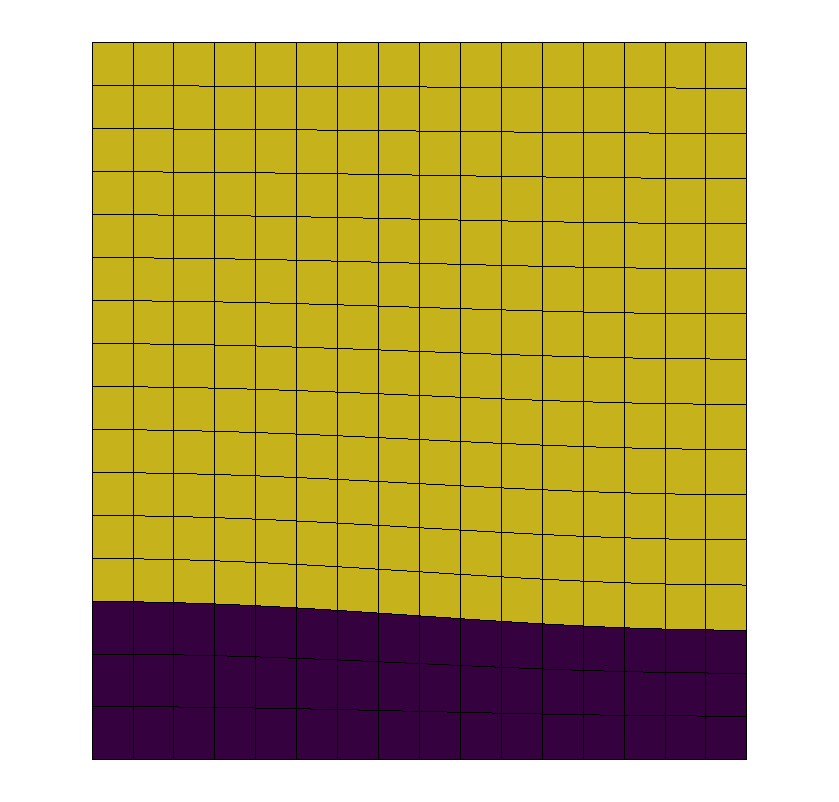
\includegraphics[width=5cm]{python_codes/fieldstone_25/results/mats}
\end{center}

The code relies on Taylor-Hood eelements ($Q_2\times Q_1$), see Section~\ref{ss:pairq2q1} and 
on $Q_2\times P_{-1}$ elements, see Section~\ref{ss:pairq2pm1}. 
It has been  benchmarked agains the Donea \& Huerta manufactured solution, see Section~\ref{mms1}.

\newpage
%..............................................................................
\paragraph{Isoviscous case - $Q_2\times Q_1$}

\begin{center}
\includegraphics[width=5.cm]{python_codes/fieldstone_25/results/100_100/vel}
\includegraphics[width=5.cm]{python_codes/fieldstone_25/results/100_100/u}
\includegraphics[width=5.cm]{python_codes/fieldstone_25/results/100_100/v}\\
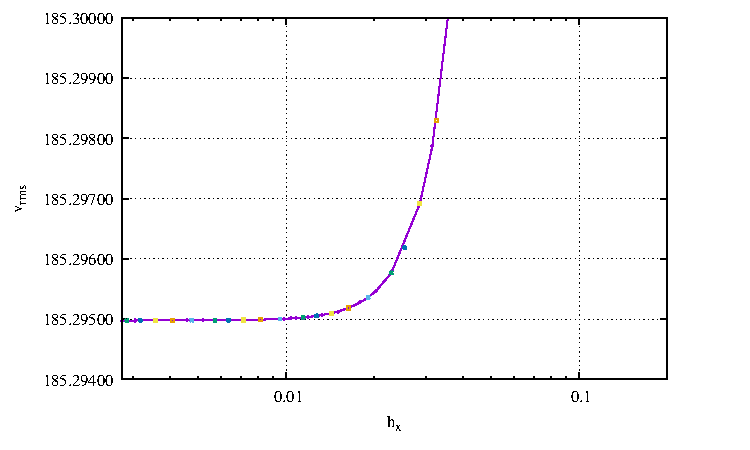
\includegraphics[width=6cm]{python_codes/fieldstone_25/results/vrms_100.pdf}
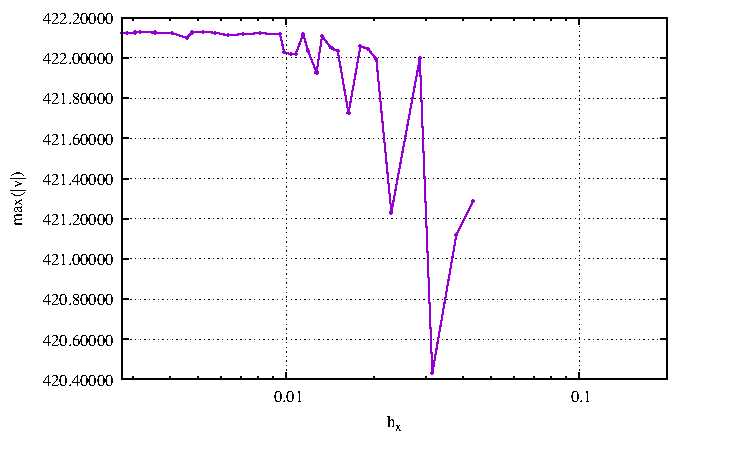
\includegraphics[width=6cm]{python_codes/fieldstone_25/results/max_vel_100.pdf}\\
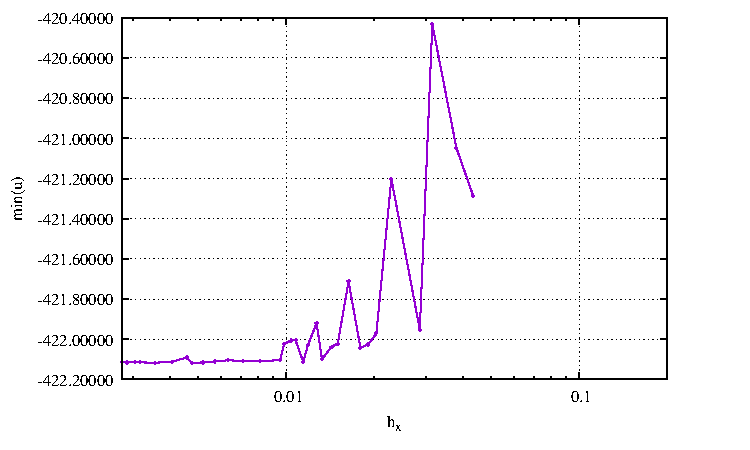
\includegraphics[width=6cm]{python_codes/fieldstone_25/results/min_u_100.pdf}
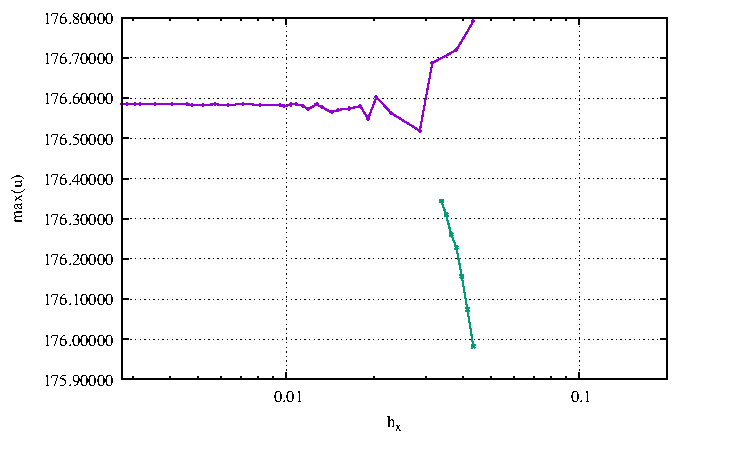
\includegraphics[width=6cm]{python_codes/fieldstone_25/results/max_u_100.pdf}\\
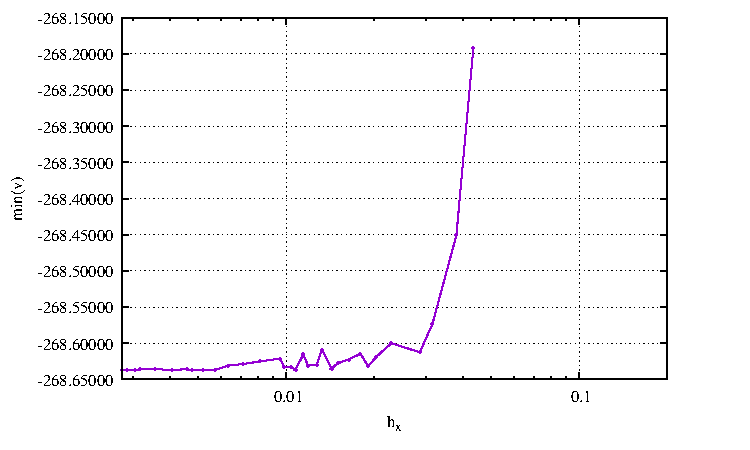
\includegraphics[width=6cm]{python_codes/fieldstone_25/results/min_v_100.pdf}
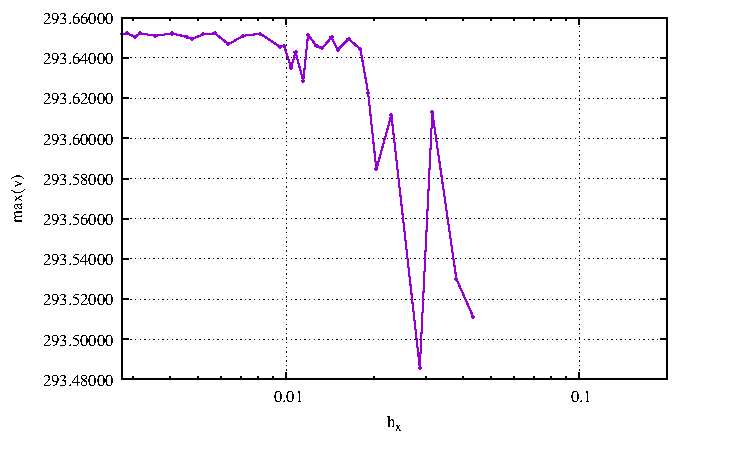
\includegraphics[width=6cm]{python_codes/fieldstone_25/results/max_v_100.pdf}\\
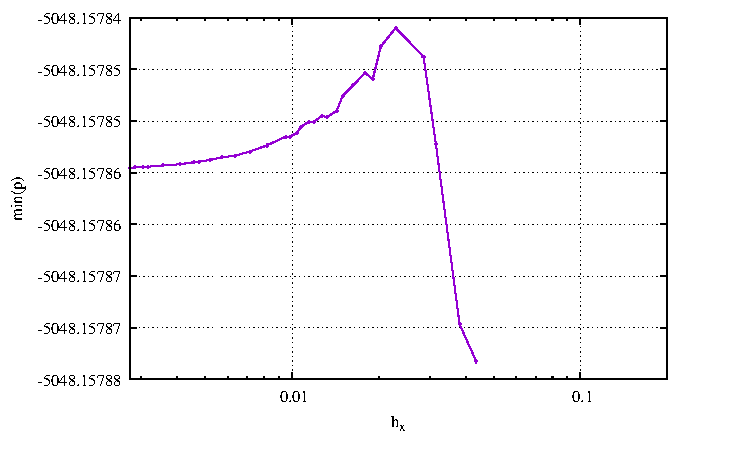
\includegraphics[width=6cm]{python_codes/fieldstone_25/results/min_p_100.pdf}
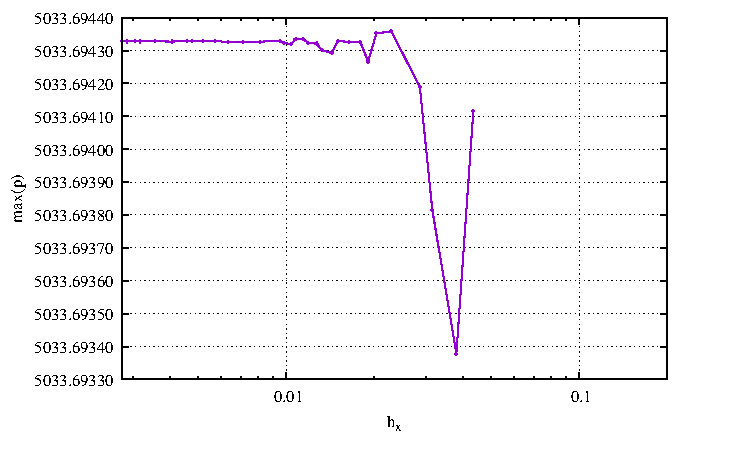
\includegraphics[width=6cm]{python_codes/fieldstone_25/results/max_p_100.pdf}\\
{\captionfont Results obtained with $Q_2\times Q_1$ elements} 
\end{center}


\begin{tabular}{lllll}
\hline
nelx & hx & $\upnu_{rms}(\times 10^{-6})$ & $\upnu^\star_{rms}(\times 10^{-6})$ (extrap.)  & rate \\
\hline\hline
25   & 0.036568 & 185.30019494838673 & 185.2949797 & 4.009763002 \\
50   & 0.018284 & 185.29530341925154 & 185.2949798 & 4.0348654   \\
100  & 0.009142 & 185.29499975286718 & X & X \\
200  & 0.004571 & 185.29498097047734 & X & X \\
\hline
8    & 0.114275      & 185.9669437569909  &  185.2954174 & 4.404188247 \\
16   & 0.0571375     & 185.32713277686372 &  185.2949839 & 4.057065851 \\
32   & 0.02856875    & 185.29691524980284 &  185.2949784 & 3.995213562 \\
64   & 0.014284375   & 185.29509989938787 &  185.2949832 & 6.637356434 \\
128  & 0.0071421875  & 185.29498605775253 &  X           & X           \\
256  & 0.00357109375 & 185.29498319303758 &  X           & X           \\
\hline
\end{tabular}

\newpage
%..............................................................................
\paragraph{Isoviscous case - $Q_2\times P_{-1}$}

All things equal, this element gives me a headache because at low resolution the velocity
field showcases a weird pattern which I cannot explain. It is immune to the number of quadrature points. 
Since the code was benchmarked against a manufactured solution for a regular and perturbed 
mesh, I don't understand what is going on.










\newpage
%..............................................................................
\paragraph{Viscosity ratio = 10 - $Q_2\times Q_1$}

\begin{center}
\includegraphics[width=5.cm]{python_codes/fieldstone_25/results/010_100/vel}
\includegraphics[width=5.cm]{python_codes/fieldstone_25/results/010_100/u}
\includegraphics[width=5.cm]{python_codes/fieldstone_25/results/010_100/v}\\
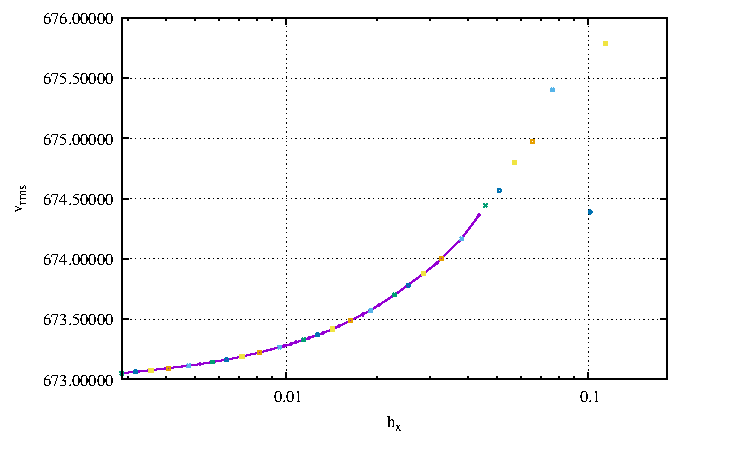
\includegraphics[width=6cm]{python_codes/fieldstone_25/results/vrms_010.pdf}
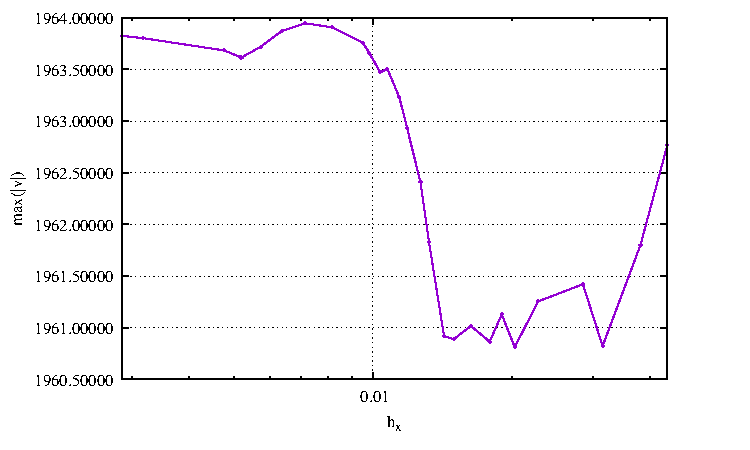
\includegraphics[width=6cm]{python_codes/fieldstone_25/results/max_vel_010.pdf}\\
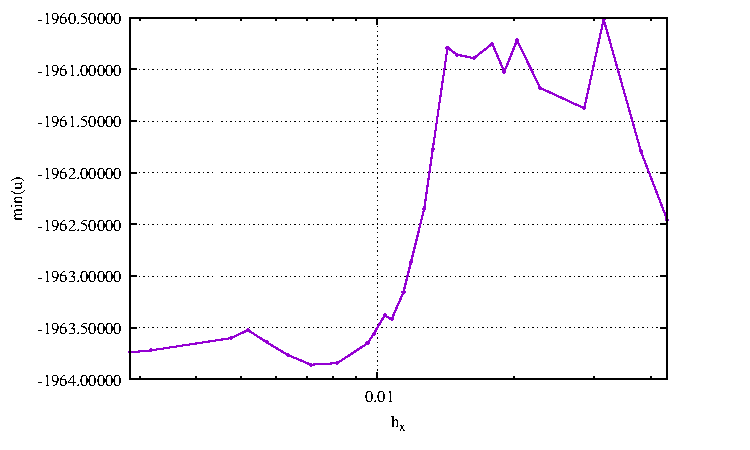
\includegraphics[width=6cm]{python_codes/fieldstone_25/results/min_u_010.pdf}
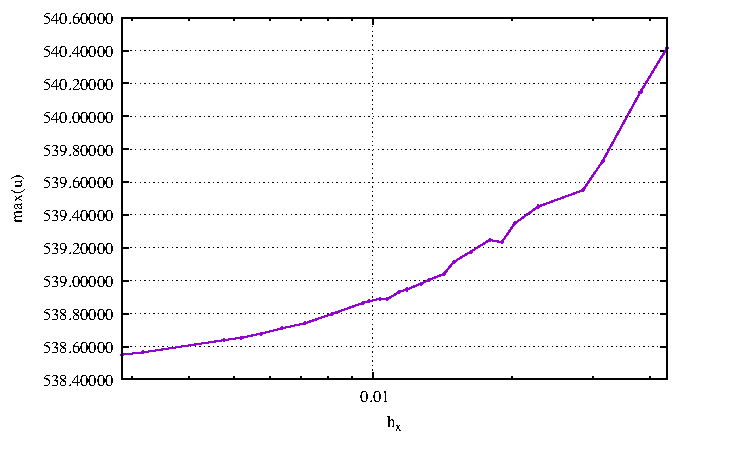
\includegraphics[width=6cm]{python_codes/fieldstone_25/results/max_u_010.pdf}\\
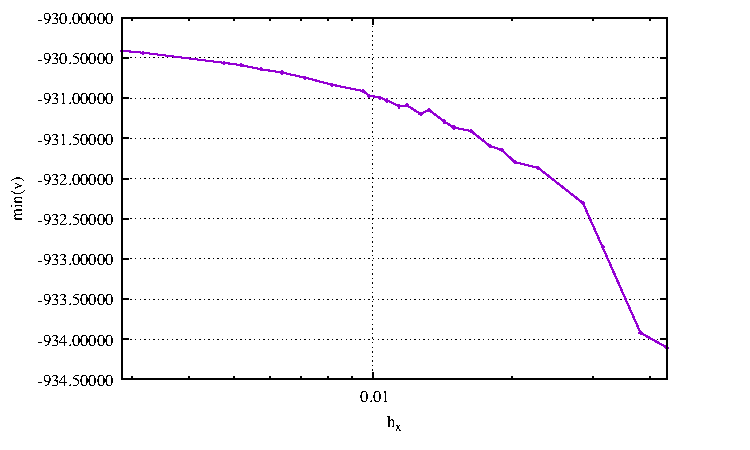
\includegraphics[width=6cm]{python_codes/fieldstone_25/results/min_v_010.pdf}
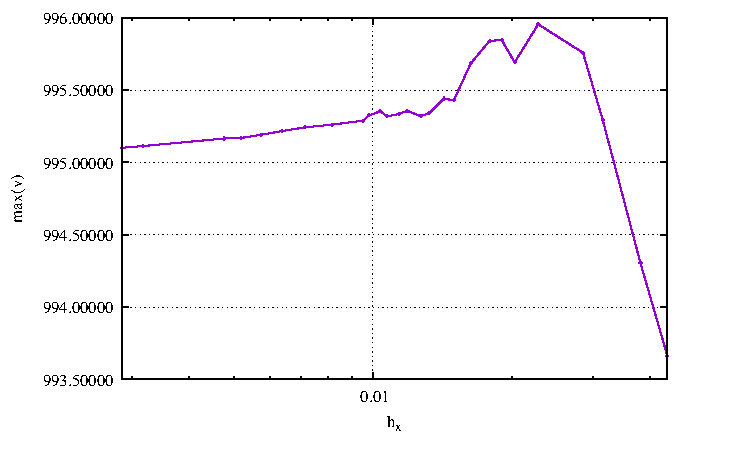
\includegraphics[width=6cm]{python_codes/fieldstone_25/results/max_v_010.pdf}\\
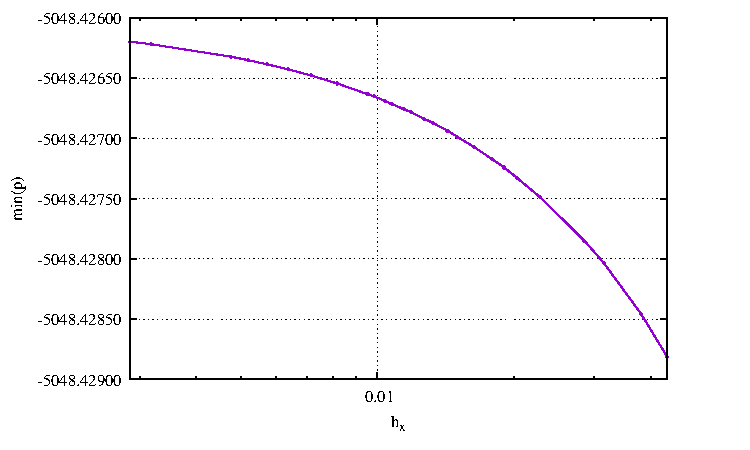
\includegraphics[width=6cm]{python_codes/fieldstone_25/results/min_p_010.pdf}
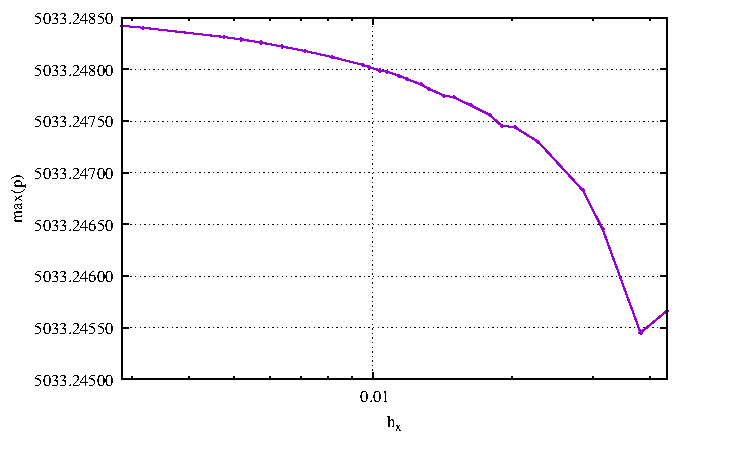
\includegraphics[width=6cm]{python_codes/fieldstone_25/results/max_p_010.pdf}\\
{\captionfont Results obtained with $Q_2\times Q_1$ elements} 
\end{center}




\begin{tabular}{lllll}
\hline
nelx & hx & $\upnu_{rms}(\times 10^{-6})$ & $\upnu^\star_{rms}(\times 10^{-6})$ (extrap.)  & rate \\
\hline\hline
8    & 0.114275      & 0.0006757876577772155 & 0.0006608591144 & 0.09867640232 \\
16   & 0.0571375     & 0.0006748007227229576 & 0.0006729590166 & 1.001309003   \\ 
32   & 0.02856875    & 0.000673879034543635  & 0.0006729654426 & 1.011510945   \\
64   & 0.014284375   & 0.0006734186084028846 & X& X\\
128  & 0.0071421875  & 0.0006731902248433064 & X& X\\
256  & 0.00357109375 & 0.000673075657106445  & X& X\\
\hline
\end{tabular}












\newpage
%..............................................................................
\paragraph{Viscosity ratio = 100 - $Q_2\times Q_1$}

\begin{center}
\includegraphics[width=5.cm]{python_codes/fieldstone_25/results/001_100/vel}
\includegraphics[width=5.cm]{python_codes/fieldstone_25/results/001_100/u}
\includegraphics[width=5.cm]{python_codes/fieldstone_25/results/001_100/v}\\
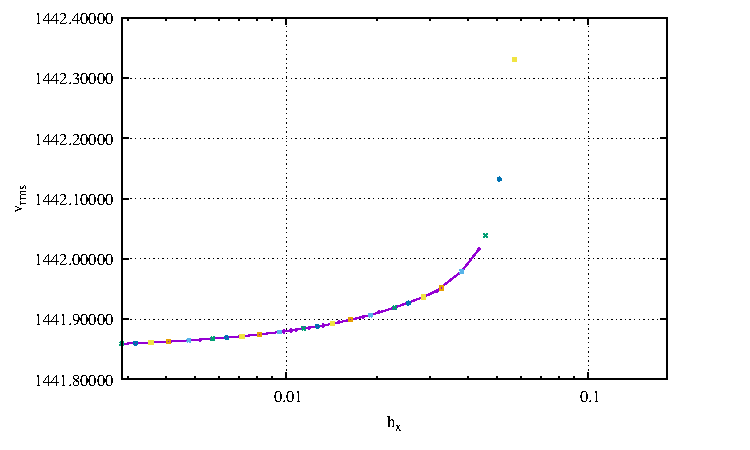
\includegraphics[width=6cm]{python_codes/fieldstone_25/results/vrms_001.pdf}
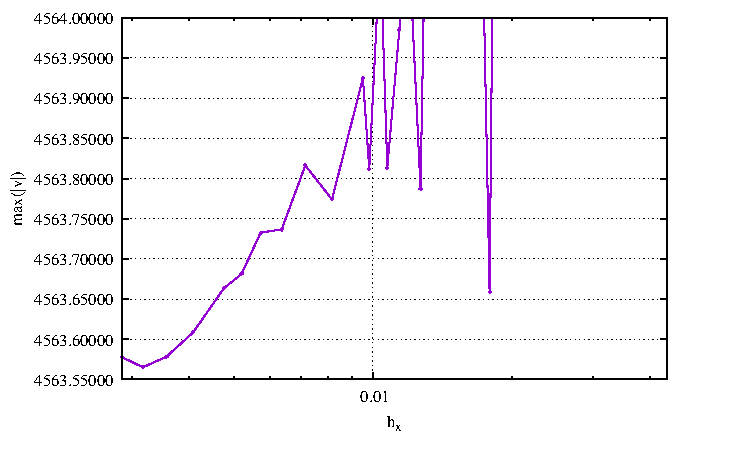
\includegraphics[width=6cm]{python_codes/fieldstone_25/results/max_vel_001.pdf}\\
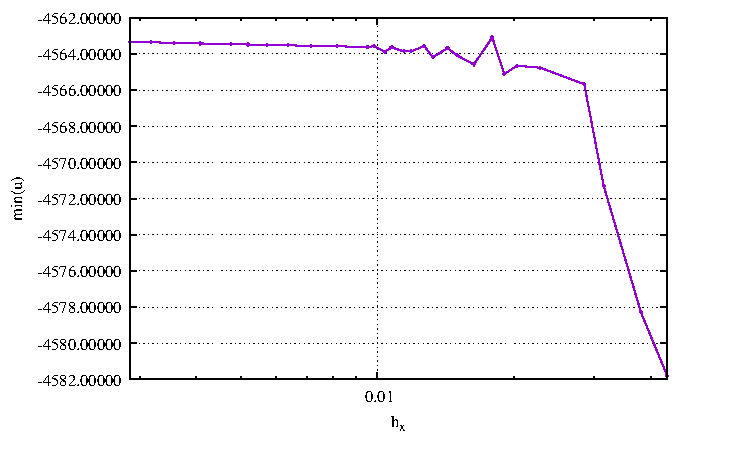
\includegraphics[width=6cm]{python_codes/fieldstone_25/results/min_u_001.pdf}
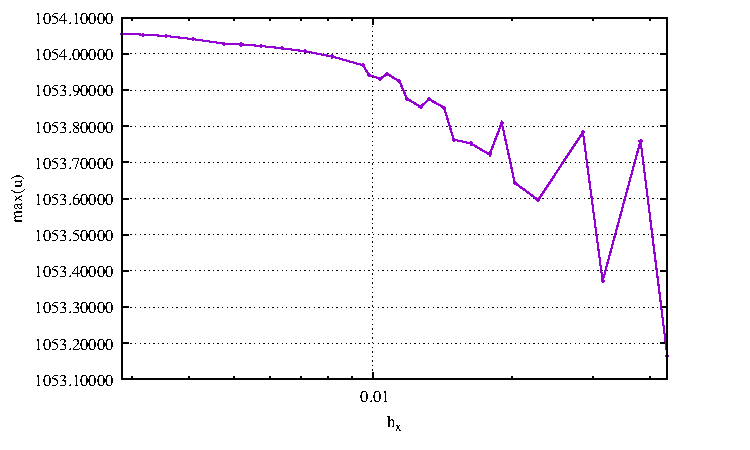
\includegraphics[width=6cm]{python_codes/fieldstone_25/results/max_u_001.pdf}\\
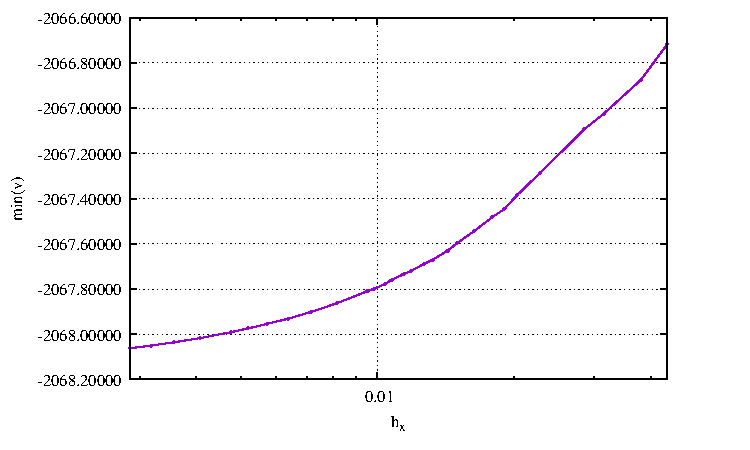
\includegraphics[width=6cm]{python_codes/fieldstone_25/results/min_v_001.pdf}
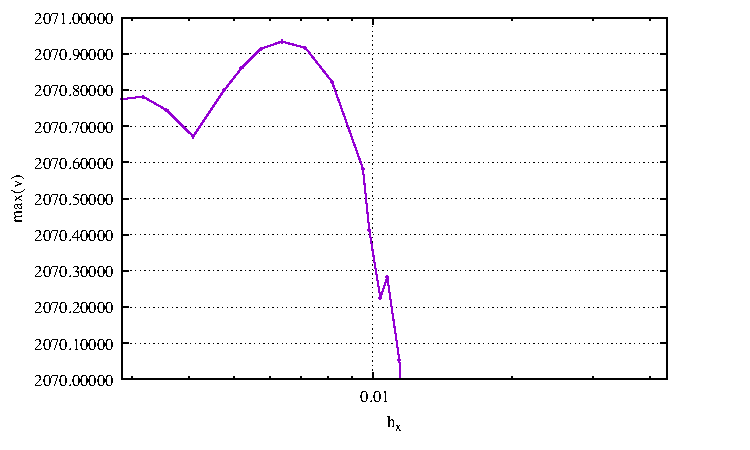
\includegraphics[width=6cm]{python_codes/fieldstone_25/results/max_v_001.pdf}\\
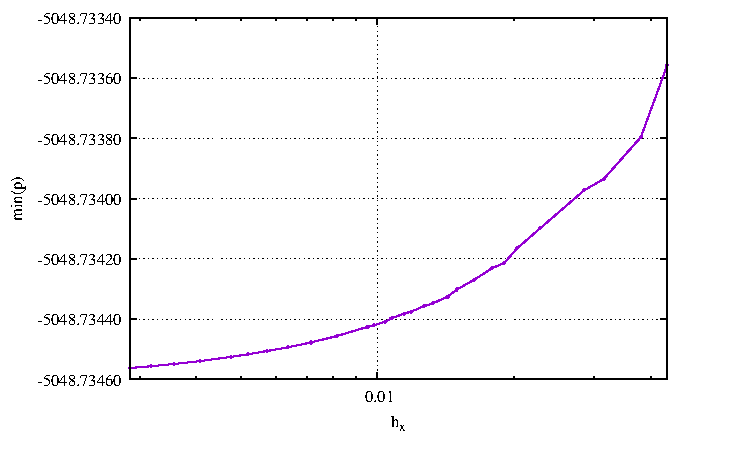
\includegraphics[width=6cm]{python_codes/fieldstone_25/results/min_p_001.pdf}
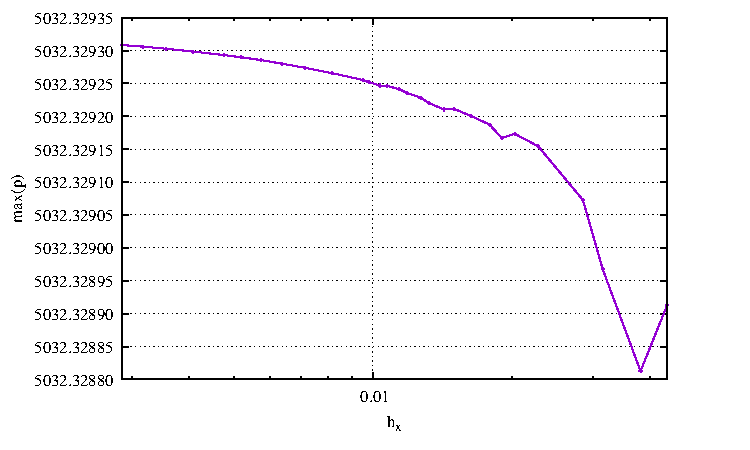
\includegraphics[width=6cm]{python_codes/fieldstone_25/results/max_p_001.pdf}\\
{\captionfont Results obtained with $Q_2\times Q_1$ elements} 
\end{center}

\begin{tabular}{lllll}
\hline
$nelx$ & $h_x$ & $\upnu_{rms}(\times 10^{-6})$ & $\upnu^\star_{rms}(\times 10^{-6})$ (extrap.)  & rate \\
\hline\hline
8    & 0.114275      & 0.0015073487507568553 &  0.001441934413 & 7.364696091 \\
16   & 0.0571375     & 0.0014423313101926754 &  0.001441886911 & 3.154474001 \\
32   & 0.02856875    & 0.0014419368207029728 &  0.0014418534   & 1.09262734 \\
64   & 0.014284375   & 0.0014418925165763435 &  X              & X   \\
128  & 0.0071421875  & 0.0014418717420808874 &  X              & X   \\
256  & 0.00357109375 & 0.0014418612856352821 &  X              & X   \\
\hline
\end{tabular}















